\begin{figure}[p]
\centering
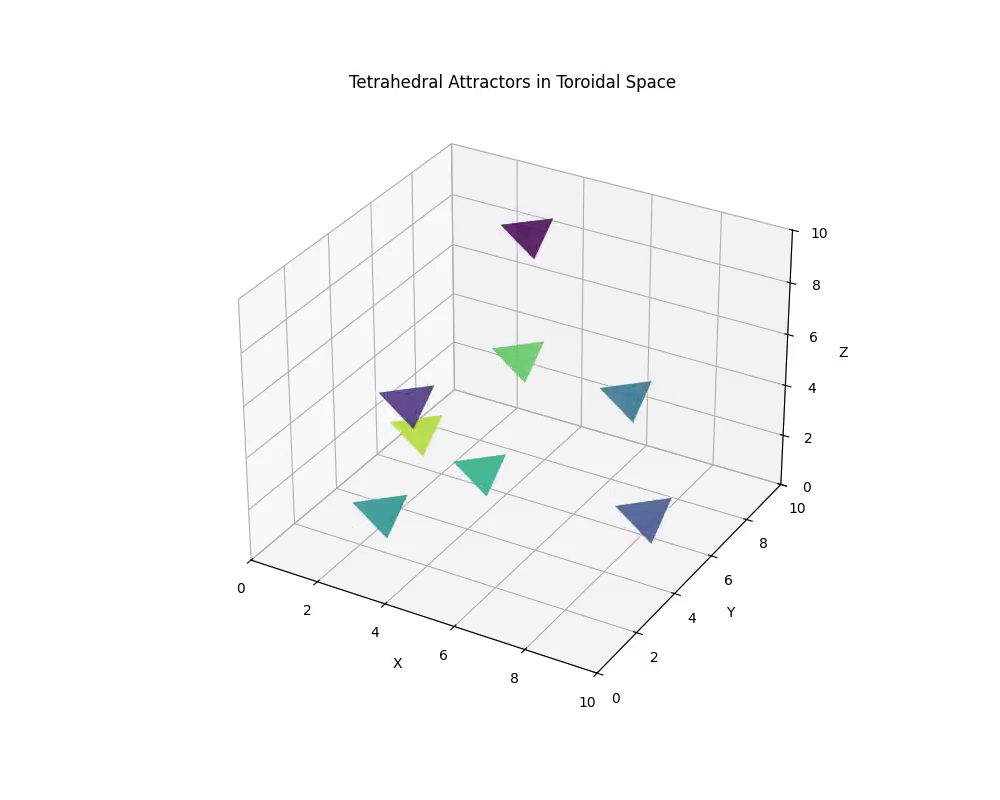
\includegraphics[width=0.485\linewidth,height=0.32\textheight,keepaspectratio]{figures/F07_0.png}
\hfill
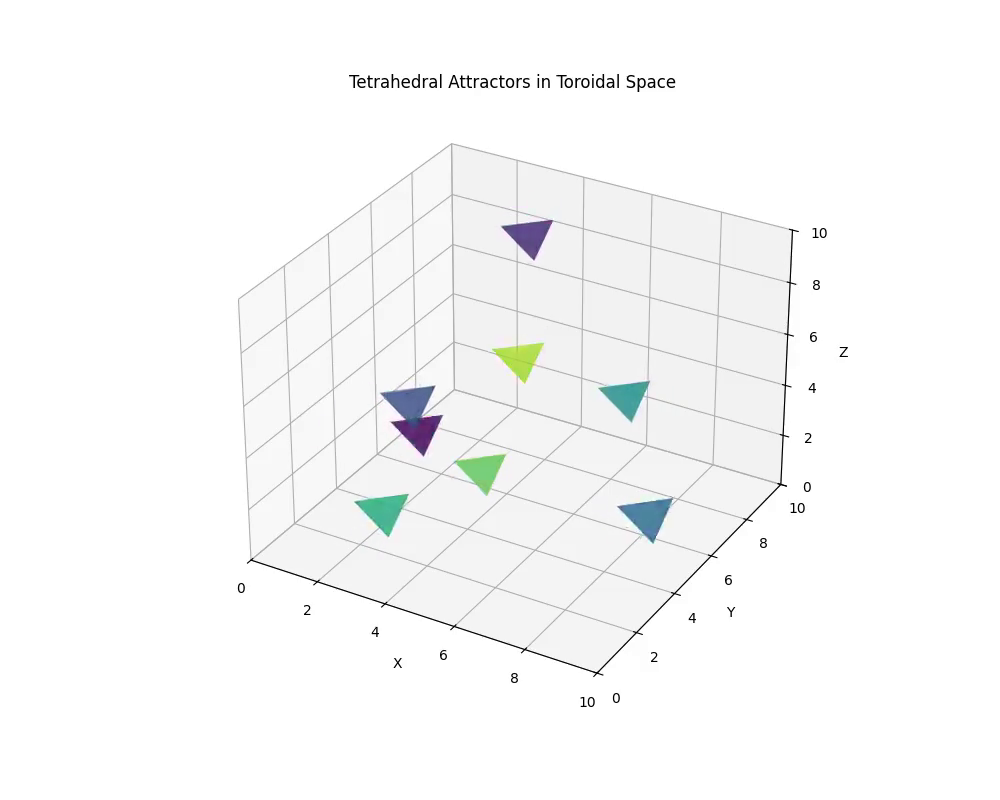
\includegraphics[width=0.485\linewidth,height=0.32\textheight,keepaspectratio]{figures/F07_1.png}
\par\medskip
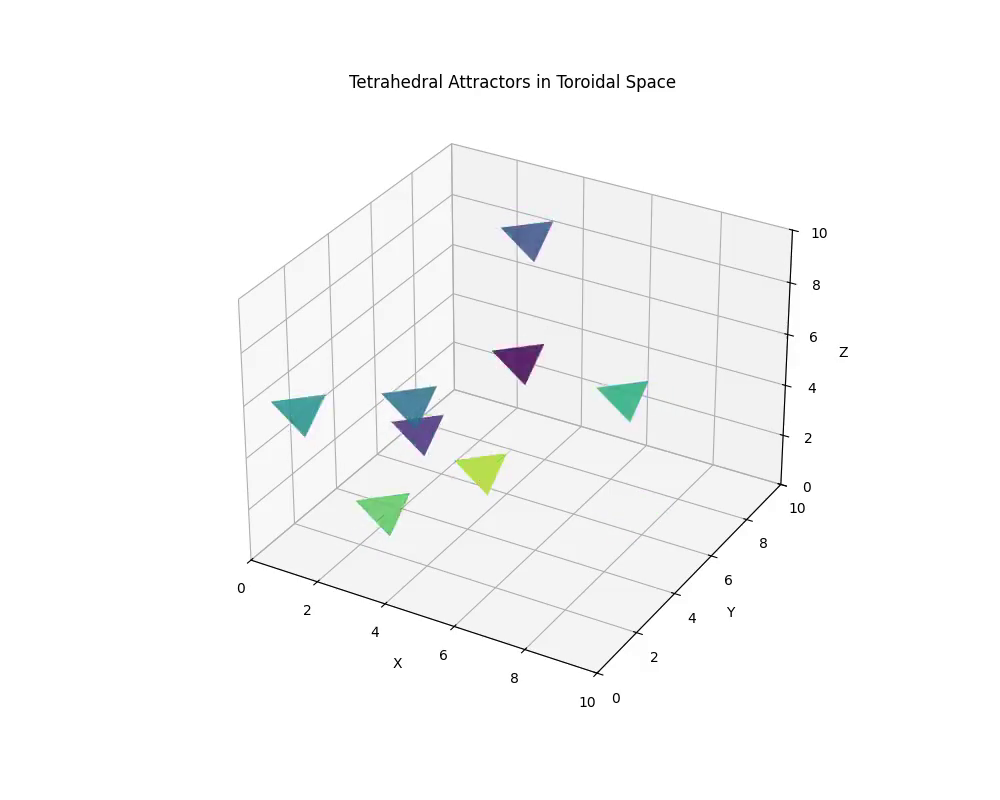
\includegraphics[width=0.485\linewidth,height=0.32\textheight,keepaspectratio]{figures/F07_2.png}
\hfill
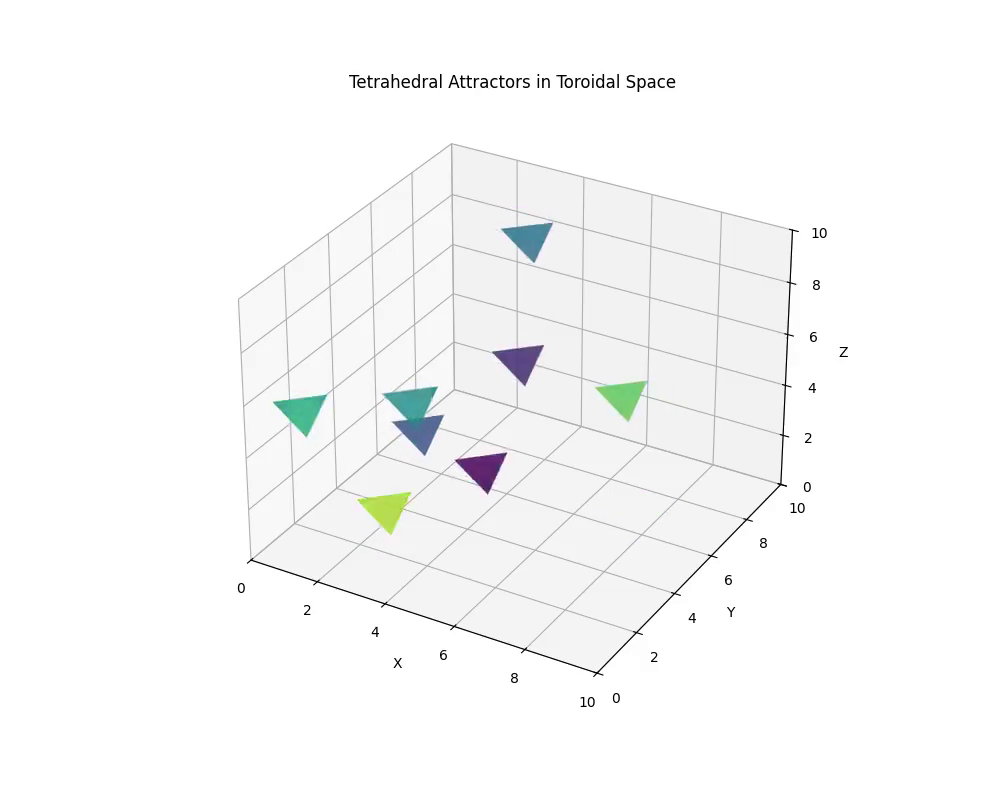
\includegraphics[width=0.485\linewidth,height=0.32\textheight,keepaspectratio]{figures/F07_3.png}
\par\medskip
\caption[The localized S02 screen relocation]{ORIGINAL movie content / ATTRIBUTED. Consecutive S02 frames 12--15 in reading order (0.2000--0.2500 movie seconds). The conspicuous relocation occurs between 13 and 14 and is consistent with wrapping. Missing numerical states prevent a certified crossing axis or native displacement. Color also advances between frames and is not a stable body label. \cite{construction02}}
\label{fig:F07}
\end{figure}
